% Begin the document and set up the style of the document
\documentclass[a4paper]{article}

% Install the required packages for the document 
\usepackage{envmath}
\usepackage{esvect}
\usepackage{graphicx}
\usepackage{gensymb}
\usepackage{tikz}
\usepackage{geometry}
\usepackage{enumitem}
\usepackage{mathtools}
\usepackage{graphicx}
\usepackage{amsmath}
\usepackage{amscd}
\usepackage{amssymb}
\usepackage{amsfonts}
\usepackage{pgf}
\usepackage{tikz}
\usepackage{mathrsfs}
\usepackage{asyalign}
\usepackage{physics}
\usepackage{cite}
\usepackage{url}
\usepackage[tableposition=top]{caption}
\usepackage{ifthen}
\usepackage[utf8]{inputenc}
\usetikzlibrary{arrows}

\begin{document}

\begin{center}
	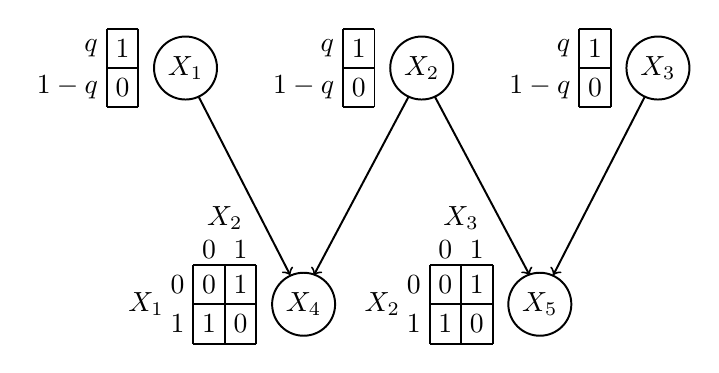
\begin{tikzpicture}

		\draw[line width = 0.25mm] (-3,3) circle (4mm);
		\node at (-3,3) {$X_1$};
		\draw[line width = 0.25mm] (0,3) circle (4mm);
		\node at (0,3) {$X_2$};
		\draw[line width = 0.25mm] (3,3) circle (4mm);
		\node at (3,3) {$X_3$};

		\draw[line width = 0.25mm] (-1.5,0) circle (4mm);
		\node at (-1.5,0) {$X_4$};
		\draw[line width = 0.25mm] (1.5,0) circle (4mm);
		\node at (1.5,0) {$X_5$};

		\draw[line width = 0.25mm][->] (-2.83,2.63) -- (-1.67,0.37);

		\draw[line width = 0.25mm][->] (-0.17,2.63) -- (-1.37,0.37);

		\draw[line width = 0.25mm][->] (0.17,2.63) -- (1.37,0.37);

		\draw[line width = 0.25mm][->] (2.83,2.63) -- (1.67,0.37);

		\draw[line width = 0.25mm] (-3.6,3) -- (-4,3);
		\draw[line width = 0.25mm] (-3.6,3.5) -- (-4,3.5);
		\draw[line width = 0.25mm] (-3.6,2.5) -- (-4,2.5);
		\draw[line width = 0.25mm] (-3.6,3.5) -- (-3.6,2.5);
		\draw[line width = 0.25mm] (-4,3.5) -- (-4,2.5);
		\node at (-3.8,3.25) {$1$};
		\node at (-3.8,2.75) {$0$};
		\node at (-4.2, 3.25) {$q$};
		\node at (-4.5, 2.75) {$1-q$};

		\draw[line width = 0.25mm] (-0.6,3) -- (-1,3);
		\draw[line width = 0.25mm] (-0.6,3.5) -- (-1,3.5);
		\draw[line width = 0.25mm] (-0.6,2.5) -- (-1,2.5);
		\draw[line width = 0.25mm] (-0.6,3.5) -- (-0.6,2.5);
		\draw[line width = 0.25mm] (-1,3.5) -- (-1,2.5);
		\node at (-0.8,3.25) {$1$};
		\node at (-0.8,2.75) {$0$};
		\node at (-1.2, 3.25) {$q$};
		\node at (-1.5, 2.75) {$1-q$};

		\draw[line width = 0.25mm] (2.4,3) -- (2,3);
		\draw[line width = 0.25mm] (2.4,3.5) -- (2,3.5);
		\draw[line width = 0.25mm] (2.4,2.5) -- (2,2.5);
		\draw[line width = 0.25mm] (2.4,3.5) -- (2.4,2.5);
		\draw[line width = 0.25mm] (2,3.5) -- (2,2.5);
		\node at (2.2,3.25) {$1$};
		\node at (2.2,2.75) {$0$};
		\node at (1.8, 3.25) {$q$};
		\node at (1.5, 2.75) {$1-q$};

		\draw[line width = 0.25mm] (-2.1,0) -- (-2.9,0);
		\draw[line width = 0.25mm] (-2.1,0.5) -- (-2.9,0.5);
		\draw[line width = 0.25mm] (-2.1,-0.5) -- (-2.9,-0.5);
		\draw[line width = 0.25mm] (-2.1,0.5) -- (-2.1,-0.5);
		\draw[line width = 0.25mm] (-2.9,0.5) -- (-2.9,-0.5);
		\draw[line width = 0.25mm] (-2.5,0.5) -- (-2.5,-0.5);
		\node at (-2.3,0.25) {$1$};
		\node at (-2.3,-0.25) {$0$};
		\node at (-2.7,0.25) {$0$};
		\node at (-2.7,-0.25) {$1$};

		\node at (-3.1, 0.25) {$0$};
		\node at (-3.1, -0.25) {$1$};
		\node at (-2.7, 0.7) {$0$};
		\node at (-2.3, 0.7) {$1$};

		\node at (-3.5, 0) {$X_1$};
		\node at (-2.5, 1.1) {$X_2$};

		\draw[line width = 0.25mm] (0.9,0) -- (0.1,0);
		\draw[line width = 0.25mm] (0.9,0.5) -- (0.1,0.5);
		\draw[line width = 0.25mm] (0.9,-0.5) -- (0.1,-0.5);
		\draw[line width = 0.25mm] (0.9,0.5) -- (0.9,-0.5);
		\draw[line width = 0.25mm] (0.1,0.5) -- (0.1,-0.5);
		\draw[line width = 0.25mm] (0.5,0.5) -- (0.5,-0.5);
		\node at (0.3,0.25) {$0$};
		\node at (0.3,-0.25) {$1$};
		\node at (0.7,0.25) {$1$};
		\node at (0.7,-0.25) {$0$};

		\node at (-0.1, 0.25) {$0$};
		\node at (-0.1, -0.25) {$1$};
		\node at (0.7, 0.7) {$1$};
		\node at (0.3, 0.7) {$0$};

		\node at (-0.5, 0) {$X_2$};
		\node at (0.5, 1.1) {$X_3$};

	\end{tikzpicture}
\end{center}

\end{document}